%!TEX root = ../Demo.tex
\chapter{绪论}

无人机(UAV)是无人航空器(UnmannedAerialVehicle)的简称,是一种不载操作人员、用空气动力产生运载工具升力、能够自主或遥控飞行、能够一次使用或回收并且载有杀伤或非杀伤有效载荷的有动力的航空器。总的来说,分为固定翼无人机、无人直升机和多旋翼无人机三大类。多旋翼无人机体积较小,成本较低,与固定翼无人机相比,具有可定点悬停、可垂直起降等优势,被应用于电力巡线、救灾探测、勘探测绘、人员搜救等用途。

在安防、救援、火情检测等方面,多旋翼飞行器正发挥誉为强大的作用,目前以DJI为主的多旋翼飞行器已经实现了包括自动起飞/航点巡航/视觉检测/自主目标追踪等功能。随着行业化应用的普及,无人机逐渐由以航拍器为主的娱乐化和影视行业发展至工业化检测等应用,并作为空中飞行平台,搭载其他行业应用负载设备,实现特定行业化功能。

在过去的几十年里,红外热成像成为工业和建筑领域的重要话题。这方面的最新发展之一是从空中进行红外热成像检测。红外热像仪与无人机相结合对检测光伏系统等热敏设备尤其有用。对于红外热成像检测领域,由于受制于无人机本身尺寸的限制,很难使用720P及更高分辨率的热成像相机,进一步导致了拍摄的热源图较为模糊,难以辨认局部细节。因此,目前主流的行业无人机普遍采用双光相机方案,即:变焦可见光相机+红外热成像相机一体化方案。利用机械或电子变焦的可见光镜头可以细致描绘视角内的影像的局部细节,进而同步查看红外热像相机的影像,两者比对后综合进行检测与分析。

根据市面上已有的成品无人机或无人机开发套件,我们发现,目前以DJI为主的行业双光无人机存在不兼容开源地面站、自有协议难以实现通用等问题。

传统的PID位置控制算法由于是基于无模型控制,随着P、I、D三个参数的变换,控制系统存在振荡或响应较慢等现象。因此,我们在PID的基础上,使用基于线性模型的预测控制算法。该算法可以有效地克服过程的不确定性、非线性和并联性,并能方便的处理过程被控变量和操纵变量中的各种约束。

因此,本课题利用DJI御2行业进阶版无人机,在自研的APP内通过使用DJI MSDK接口,将DJI MSDK协议信息转换至MAVLink UDP协议帧信息,并利用无人机端侧遥控器通过以太网数据链路远程组网传输至Windows端侧QGroundControl软件。

由于国内外以开源为主的飞行器大多采用以MAVLink协议为主的通信解决方案,因此该方案可实现将DJI系列飞行器与开源飞行器进行地面站统一化管理与云上部署,显著地提升了飞行器间的兼容性与可靠性。

无人机根据MAVLink地面站给出的GPS航点信息进行航点飞行,飞行任务结束后,检测部分使用基于OpenCV霍夫圆特征检测+自适应阈值,控制部分LMPC PID位置控制实现自主视觉引导降落至特定降落目标点,并在地面站端在QGroundControl软件上利用基于YoloV5深度学习的目标检测算法实时进行可见光与热成像目标检测与异常图像分析。

\chapter{相关背景}
\section{飞控平台}

20世纪以来,随着飞行控制算法技术和飞行控制硬件的发展,无人飞行器技术使传统的地面检测技术得以拓展,进入了空中检测的时代并随着算法和硬件的不断升级而快速发展。其中,国内有以DJI为主的行业级多旋翼飞行器以及配套的司空地面站平台,也有国外以开源为主的平台(如APM、PIX飞控系统和对应的QGroundControl、MissionPlanner等开源地面站),以及由国内其他公司研发与设计的基于STM32或TI嵌入式芯片为主的简易平台(如无名飞控、匿名飞控以及其他相关平台)。

如下对比介绍了一些知名的配套平台:

1.DJI-商业多旋翼飞行器平台。对于整机飞行系统,DJI采用御/晓/精灵/经纬等系列无人机,搭配DJI GO系列APP实现遥控器端控制飞行以及相关飞行参数获取和控制拍照摄影等。DJI不提供针对于个人用户的电脑端配套地面站、云服务以及相关技术支持。对于企事业单位,DJI提供以司空系统为主的飞行器管理平台。提供基本的多无人机控制功能以及DJI官方提供的云上解决方案,不提供开发接口,无法进行定制化开发与服务,并且由于司空系统的封闭性,对于云端也同样无法进行开发。

2.Ardupilot/PX4-开源地面站平台。Ardupilot和PX4是两大主流开源无人机系统,前者由DroneCode基金会维护,后者由Auterion公司维护,Ardupilot历史要远长于PX4,因此功能更丰富,经历的坑也更多,填的坑也更多,因此有“功能完善、运行稳定”的优势。APM与PX4在一些关键算法上是相互借鉴的,因此算法先进程度差不多。PX4由于起步晚,历史包袱少,最初就搭建了一个很先进的架构,因此获得了代码简洁易懂易懂的优势。该开源系统在国内外影响力较大,除多旋翼外同样支持固定翼、垂直起降等机型。

3.STM32/TI-嵌入式芯片飞控平台。该系列以匿名、无名飞控为主,最初是由大学生创业团队设计并开发的,具有光流定位、GPS定点等功能。只支持多旋翼系列机型,并且由于其配套地面站程序较为简易,主要适用于教学实验等领域,不适用于商业等对稳定性要求较高的环境中。

\section{视觉检测}

根据项目需求,无人机检测地面上面的H标记采用基于OpenCV的框架,算法使用自适应阈值+开闭运算+霍夫圆检测,并返回检测的中心点,用于滤波以及后续的位置优化。

\subsection{霍夫圆检测}

1.霍夫变换

霍夫变换于1962年由Paul Hough ⾸次提出,后于1972年由Richard Duda和Peter Hart推⼴使⽤,经典霍夫变换⽤来检测图像中的直线,后来霍夫变换扩展到任意形状物体的识别,多为圆和椭圆。

霍夫变换 ( Hough Transform, HT)是模式识别领域中对⼆值图像进⾏直线检测的有效方法。

\begin{figure}[ht]
  \centering
  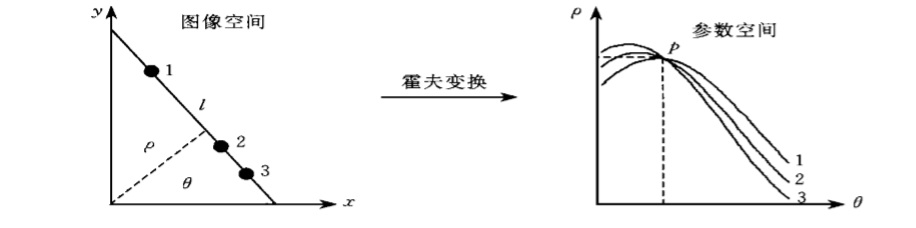
\includegraphics[width=0.8\linewidth]{./Figure/Hough_Transform.png}
  \caption{霍夫变换示意}\label{Fig:xd1}
\end{figure}

在标准参数化方式下 ,图像空间中的直线 l 的表达为:

$d=x \cos \theta+y \sin \theta, \quad d \geqslant 0,0 \leqslant \theta<\pi$

右边的图意思是在⼀个点上,不同的θ 对应不同的ρ,θ是穿过该点的直线的斜率,ρ是穿过该点的直线与原点的距离。这样穿过每个点 作⽆数条直线,参数ρ和θ就能绘出⼀个正弦图像。 ⽽如果1,2,3在⼀条直线上就可以找到⼀个θ使得过1,2,3点的直线的ρ很接近。也就是有图上相交的过程。而通常使⽤的方法是累加法,求得累加次数最多的(θ,ρ)从⽽确定这条直线。

2.霍夫变换用于圆检测

与使用(r,theta)来表示⼀条直线相似,使⽤(a,b,r)来确定⼀个圆心为(a,b)半径为r的圆。

某个圆过点(x1,y1),则有:$(x1-a1)^2 + (y1-b1)^2 = r1^2$

那么过点(x1,y1)的所有圆可以表⽰为(a1(i),b1(i),r1(i)),其中r1∈(0,⽆穷),每⼀个 i 值都对应⼀个不同的圆, (a1(i),b1(i),r1(i))表⽰了⽆穷多个过点(x1,y1)的圆。

过点(x1,y1)的所有圆可以表⽰为(a1(i),b1(i),r1(i)),过点(x2,y2)的所有圆可以表⽰为(a2(i),b2(i),r2(i)),过点 (x3,y3)的所有圆可以表⽰为(a3(i),b3(i),r3(i)),如果这三个点在同⼀个圆上,那么存在⼀个值(a0,b0,r0),使得 a0 = a1(k)=a2(k)=a3(k) 且b0 = b1(k) = b2(k) = b3(k) 且r0=r1(k)=r2(k)=r3(k),即这三个点同时在圆(a0,b0,r0)上。

从下图可以形象的看出:

\begin{figure}[ht]
  \centering
  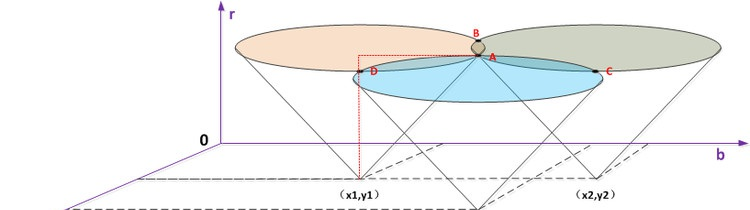
\includegraphics[width=0.8\linewidth]{./Figure/Hough_Circle.png}
  \caption{霍夫圆示意}\label{Fig:xd1}
\end{figure}

⾸先,分析过点(x1,y1)的所有圆(a1(i),b1(i),r1(i)),当确定r1(i)时 ,(a1(i),b1(i))的轨迹是⼀个以(x1,y1,r1(i))为中心半径为 r1(i)的圆。那么,所有圆(a1(i),b1(i),r1(i))的组成了⼀个以(x1,y1,0)为顶点,锥角为90度的圆锥⾯。三个圆锥面的交点A即是同时过这三个点的圆。累加次数最多的A点就是一个圆⼼。

\section{滤波优化}

对于上一步每一次检测到的降落板中心点,我们采用卡尔曼滤波器去除检测中心点的噪声并实现较为精确的降落点预测。

\subsection{卡尔曼滤波器}

卡尔曼滤波(Kalman filtering, KF)是一种利用线性系统状态方程,通过系统输入输出观测数据,对系统状态进行最优估计的算法。卡尔曼滤波的一个典型实例是从一组有限的,对物体位置的,包含噪声的观察序列中预测出物体的坐标位置及速度。在很多工程应用(雷达、计算机视觉)中都可以找到它的身影。同时,卡尔曼滤波也是控制理论以及控制系统工程中的一个重要话题。

卡尔曼滤波最早可以追溯到Wiener滤波,不同的是卡尔曼采用状态空间来描述它的滤波器,卡尔曼滤波器同时具有模糊/平滑与预测功能,特别是后者在视频分析与对象跟踪应用场景中被发扬光大,在离散空间(图像或者视频帧)使用卡尔曼滤波器相对简单。假设我们根据一个处理想知道一个变量值如下:

$x_{k+1}=\Phi x_{k}+w_{k}$

其中 $x_{k}$ 是在 $\mathrm{k}$ 时刻的状态,$\Phi$ 是从 $\mathrm{k}$ 到 $\mathrm{k}+1$ 时刻的变换矩阵,$w_{k}$ 是 $\mathrm{k}$ 时亥相关白噪声的协方差矩阵。

对观测值建模如下:

$z_{k}=H x_{k}+v_{k}$

其中 $z_{k}$ 是在 $k$ 时刻对 $x$ 的实际测量值,$\mathrm{H}$ 是状态矩阵与测量矩阵无噪声链接,$\mathrm{v}_{\mathrm{k}}$ 是测量错误

这样就得到两个协方差矩阵

$$
\begin{aligned}
&Q=E\left[w_{k} w_{k}^{T}\right] \\
&R=E\left[v_{k} v_{k}^{T}\right] \\
&P_{k}=E\left[e_{k} e_{k}^{T}\right]=E\left[\left(x_{k}-\hat{x}_{k}\right)\left(x_{k}-\hat{x}_{k}\right)^{T}\right]
\end{aligned}
$$

假设 $\hat{x}_{k}$ 前一个评估为 $\hat{x}_{k}^{\prime}$, 可以得到
$$
\hat{x}_{k}=\hat{x}_{k}^{\prime}+K_{k}\left(z_{k}-H \hat{x}_{k}^{\prime}\right)
$$

其中 $K_{k}$ 被称为卡尔曼增益, 有了它就可以更新测量模型,从而更新状态空间的下个预测。

\section{控制算法}

根据项目需求,无人机需要在自主航点飞行完毕后自主降落至指定区域,指定降落区域地面上贴有标记为H的橙红色降落板。自主降落下降阶段我们改进了传统的基于PID的控制方案,通过采用基于MPC的控制方案对控制参数进行自适应优化,从而使得降落控制阶段更为平稳。

\subsection{PID控制}

PID控制应该算是应用非常广泛的控制算法了。小到控制一个元件的温度,大到控制无人机的飞行姿态和飞行速度等等,都可以使用PID控制。PID(proportion integration differentiation)其实就是指比例,积分,微分控制,它具有原理简单,易于实现,适用面广,控制参数相互独立,参数的选定比较简单等优点;而且在理论上可以证明,对于过程控制的典型对象──“一阶滞后+纯滞后”与“二阶滞后+纯滞后”的控制对象,PID控制器是一种最优控制。

\begin{figure}[ht]
  \centering
  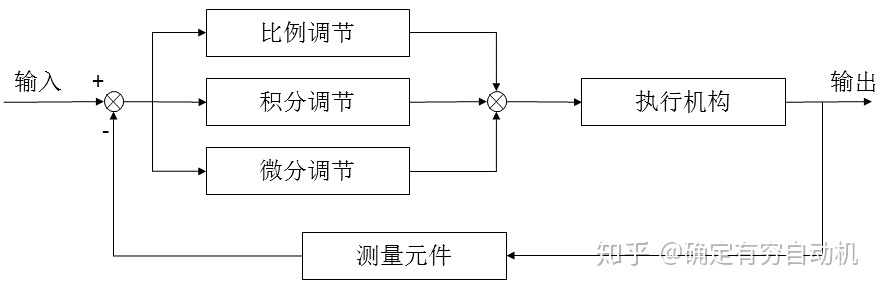
\includegraphics[width=0.8\linewidth]{./Figure/PID_Graph.jpg}
  \caption{PID控制系统结构图}\label{Fig:xd1}
\end{figure}

根据上图所示,PID控制即为:当得到系统的输出后,将输出经过比例,积分,微分3种运算方式,叠加到输入中,从而控制系统的行为。

在工业过程中,连续控制系统的理想PID控制规律为:

$u(t)=K_{p}\left(e(t)+\frac{1}{T_{t}} \int_{0}^{t} e(t) d t+T_{D} \frac{d e(t)}{d t}\right)$

式中,Kp为比例增益,比例度成倒数关系;Tt为积分时间常数;TD为微分时间常数;u(t)为PID控制器的输出信号;e(t)为给定值r(t)与测量值之差。

\subsection{MPC控制}

1.MPC控制介绍

传统PID算法的缺点是,对于系统的状态变化,控制器的输出不能很好的控制系统的状态变化,因此,在这种情况下,PID算法的效率不高。而MPC算法则是一种更好的控制方法,它能够更好的控制系统的状态变化,并且能够更好的控制系统的输出。

模型预测控制(Model predictive control、MPC)是过程控制中,在满足特定限制条件时,控制过程的进阶控制方式,自1980年代起已用在化学工厂及炼油厂的工业过程中。模型预测控制是以过程的动态模型为基础,多半是透过系统识别得到的线性经验模型。模型预测控制的特点是每一次针对目前的时间区块内作最佳化,然后下一个时间再针对时间区块内作最佳化,这和LQR控制器不同。模型预测控制可以预测未来事件并且进行对应的处理,而传统的PID控制器没有这样的预测功能。预测控制打破了传统控制中对模型结构的严格要求,更着重于在系统已获取的信息的基础上根据功能要求按照最方便的途径建立模型。尽管模型预测控制形式多种多样,但都依赖下述三项基本原理:

1.1 预测模型

预控制是一种基于模型的控制算法,这一校型称为预测模型·对于预测控制来讲,只注重模型的功能,而不注重模型的形式,预测模型的功能就是能根据对象的历史信息和未来输入预其未来输出。从方法的角度讲,只要是具有预测功能的信息集合,不论其有什么样的表现形式,均可作为预测模型。因此,状态方程,传递函数这类传统的模型都可以作为预测模型。

1.2 滚动优化

预测控制的最主要特征是在线优化。预测控制这种优化控制算法是通过某一性能指标的最优来确定未来的控制作用的。这一性能指标涉及到系统未来的行为,例如,通常可取对象输出在未来的采样点上跟踪某一期望轨迹的方差最小.但也可取更广泛的形式,要求控制能量为最小而同时保持输出在某一给定范围内等。性能指标中涉及到的系统未来的行为,是根据预测模型由未来的控制策略决定的。

1.3 反馈校正

预控制算法在进行滚动优化时,优化的基点应与系统实际一致。但作为基础的预测模型,只是对象动态特性的粗略描述,由于实际系统中存在的非线性、时变、模型失配、干扰等因素,基于不变模型的预测不可能和实际情况完全相符,这就需用要用附加的预测手段补充模型预的不足,或者对基础模型进行在线峰正。滚动优化只有建立在反馈校正的基础上,才能体见出其优越性。因此,预测控制算法在通过优化确定了一系列末来的控制作用后,为了防止模型失配或环境干扰引起控制对理想状态的偏离,并不是把这些控制作用逐一全部实施,而只是实现本时刻的控制作用。到下一采样时刻,则首先检测对象的实际输出,并利用这一实时信息对基于模型的预测进行修正,然后再进行新的优化。

以下方框图提供了MPC原理的可视化表示:

\begin{figure}[ht]
  \centering
  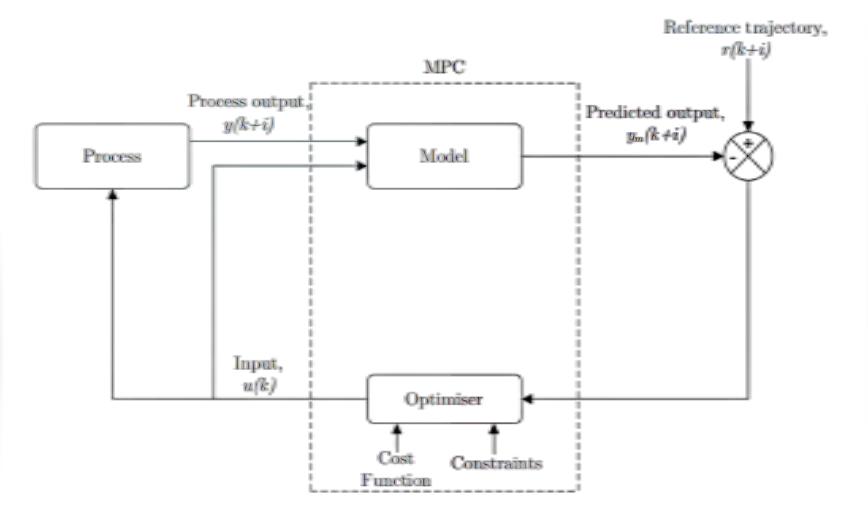
\includegraphics[width=0.8\linewidth]{./Figure/MPC-Control.png}
  \caption{MPC控制系统结构图}\label{Fig:xd1}
\end{figure}

以下图说明了MPC中的预测范围:

\begin{figure}[ht]
  \centering
  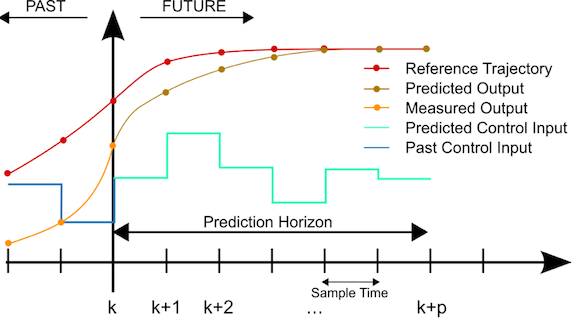
\includegraphics[width=0.8\linewidth]{./Figure/MPC-Prediction.png}
  \caption{MPC预测范围}\label{Fig:xd1}
\end{figure}

2.MPC控制系统控制器建模

对于以下控制模型:

$$
x(k+1)=A x(k)+B u(k)
$$

写成矩阵格式:

$$
\left[\begin{array}{l}x_{1}(k+1) \\x_{2}(k+1)\end{array}\right]=\left[\begin{array}{cc}1 & 0.1 \\0 & 2\end{array}\right]\left[\begin{array}{l}x_{1}(k) \\x_{2}(k)\end{array}\right]+\left[\begin{array}{c}0 \\0.5\end{array}\right] u(k)
$$

此处的$x_{1}$和$x_{2}$可以理解为误差项

$X(k)=\left[\begin{array}{c}x(k \mid k) \\x(k+1 \mid k) \\\vdots\\ x(k+j \mid k)\\\vdots \\x(k+N \mid k)\end{array}\right]$$U(k)=\left[\begin{array}{c}u(k \mid k) \\u(k+1 \mid k) \\\vdots\\ u(k+i \mid k)\\\vdots \\u(k+N-1 \mid k)\end{array}\right]$

对于MPC矩阵:

$$
x_{k}=M x_{k}+C u_{k}
$$

$M=\left[\begin{array}{c}I_{n \times n} \\A_{n \times n} \\A_{n}^{2} \\\vdots \\A^{N}\end{array}\right]$$C=\left[\begin{array}{cccc}
0 & 0 & \ldots & 0 \\
& \vdots & \ldots & \vdots \\
\vdots & 0 & & 0 \\
0 & & 0 & \ldots & 0 \\
B_{n \times p} & 0 & \ldots & 0 \\
A B_{n \times p} & B & \vdots & 0 \\
\vdots & \vdots & & B
\end{array}\right]$

$X(k)=\left[\begin{array}{c}x(k \mid k) \\x(k+1 \mid k) \\x(k+2 \mid k) \\x(k+3 \mid k)\end{array}\right]=\left[\begin{array}{c}x_{1}(k \mid k) \\x_{2}(k \mid k) \\x_{1}(k+1 \mid k) \\x_{2}(k+1 \mid k) \\x_{1}(k+2 \mid k) \\x_{2}(k+2 \mid k) \\x_{1}(k+3 \mid k) \\x_{2}(k+3 \mid k)\end{array}\right]$

$U(k)=\left[\begin{array}{c}u(k \mid k) \\u(k+1 \mid k) \\u(k+2 \mid k)\end{array}\right]=\left[\begin{array}{c}\frac{u(k \mid k)}{u(k+1 \mid k)} \\u(k+2 \mid k)\end{array}\right]$

计算出M矩阵和C矩阵

之后构建二次规划模式(cost function)

$$
J=\sum_{k=0}^{N-1} x(k+i \mid k)^{T} Q x(k+i \mid k)+u(k+i \mid k)^{T} R u(k+i \mid k)+x(k+N \mid k)^{T} F x(k+i \mid k)
$$

Q、R、F表示对应输入输出的权重系数矩阵

Q矩阵影响x变量的相关性,R矩阵跟输入相关,F矩阵跟终值相关

$x(k+N \mid k)^{T} F x(k+i \mid k)$与系统对应的终值状态相关

简化上面的 cost function 矩阵

$$
J=\boldsymbol{x}(k)^{T} \boldsymbol{G} \boldsymbol{x}(k)+\boldsymbol{U}(k)^{T} \boldsymbol{H} \boldsymbol{U}(k)+2 \boldsymbol{x}(k)^{T} \boldsymbol{E} \boldsymbol{U}(k)
$$

该矩阵只包含了输入项和已知的初始输入项x(k)

$$
\begin{aligned}&G=M^{T} \bar{Q} M \\&E=C^{T} \bar{Q} M \\&H=C^{T} \bar{Q} C+\bar{R}\end{aligned}
$$

$\bar{Q}$和$\bar{R}$表示上面式子中的Q和R矩阵的增广形式

G、H、E矩阵跟上面的M和C矩阵相关

$$
\overline{\boldsymbol{Q}}=\left[\begin{array}{ccc}\boldsymbol{Q} & \cdots & \\\vdots & \boldsymbol{Q} & \vdots \\& \cdots & \boldsymbol{F}\end{array}\right] \quad \overline{\boldsymbol{R}}=\left[\begin{array}{ccc}\boldsymbol{R} & \cdots & \\\vdots & \ddots & \vdots \\& \cdots & R\end{array}\right]
$$

\chapter{项目内容}

\section{项目概要}

本项目使用大疆御2行业进阶版无人机作为主体,基于DJI MSDK进行二次开发,对DJI MSDK自有的协议转换为兼容QGC地面站的MAVLink协议,并通过无人机端侧带屏遥控器通过以太网数据链路远程组网传输信息至远端的QGC地面站软件,以及可见光和热成像视频流信息。无人机根据地面站给出的航点信息完成航点飞行,任务结束后,云台自动向下旋转90度,并利用OpenCV计算机视觉库完成自适应阈值+开闭运算+霍夫圆检测,自主视觉引导降落至特定降落目标点,进一步在QGC地面站端利用基于YoloV5深度学习的目标检测算法实时进行可见光与热成像目标检测与异常图像分析。

\section{OpenCV视觉检测}

使用DJI的codecManager函数获取H.264的RGBA原始视频,并将获取到的每一帧新建一个Mat类型的矩阵,用于后续处理。之后利用cvtColor函数将该帧图像的RGB色彩通道转化为灰度图像,之后进行闭运算并利用findContours函数寻找图像的轮廓,寻找到轮廓后,利用drawContours函数将轮廓绘制出来,最后将图像转化为Mat类型的矩阵,并将其存入一个vector类型的容器中,最后进行霍夫圆检测。

OpenCV实现的是⼀个比标准霍夫圆变换更为灵活的检测方法——霍夫梯度法,该方法运算量相对于标准霍夫圆变换大大减少。其检测原理是依据圆心一定是在圆上的每个点的模向量上,这些圆上点模向量的交点就是圆⼼,霍夫梯度法的第一步就是找到这些圆心,这样三维的累加平⾯就又转化为二维累加平⾯。第二步是根据所有候选中心的边缘非0像素对其的支持程度来确定半径。

具体实现方法如下:

1.对于drawContours函数绘制的边缘图像,对其中的每⼀个非零点,考虑其局部梯度,即用Sobel()函数计算x和y方向的Sobel⼀阶导数得到梯度。

2.利用得到的梯度,由斜率指定的直线上的每⼀个点都在累加器中被累加,这⾥的斜率是从⼀个指定的最小值到指定的最大值的距离。

3.同时,标记边缘图像中每⼀个非0像素的位置。

4.然后从二维累加器中这些点中选择候选的中心,这些中心都大于给定阈值并且⼤于其所有近邻。这些候选的中⼼按照累加值降序排列,以便于最支持像素的中心首先出现。

5.接下来对每⼀个中心,考虑所有的非0像素,并把这些像素按照其与中心的距离排序。从到最大半径的最小距离算起,选择非0像素最支持的⼀条半径。

6.如果⼀个中心收到边缘图像⾮0像素最充分的支持,并且到前期被选择的中心有足够的距离,那么它就会被保留下来。

\section{卡尔曼滤波与优化}

OpenCV中有两个版本的卡尔曼滤波方法:KalmanFilter(C++)和CvKalman,这里我们使用前者方案。由上一步逐帧检测得到的中心点作为待估计的状态点传入卡尔曼滤波器中,并将最优估计后的结果传出作为MPC控制的输入。

卡尔曼滤波器具体实现方法如下:

1.初始化相关参数:根据需要,定义转移矩阵A与测量矩阵H,过程噪声Q与测量噪声R,最小均方误差P,系统初始状态x(0)与初始测量值z(0)

2.预测模型:利用KF.predict()函数,返回的是下一时刻的状态值KF.statePost(k+1)

3.更新上一步的测量值measurement

4.更新卡尔曼增益量KF.correct(measurement),最终的结果应该是更新后的状态估计statePost

\section{MPC位置控制}

我们提出的四轴飞行器模型预测器位置控制如下图方框中所示:在MPC控制中,每个优化回路开始前,使用四轴飞行器状态空间模型来增强当前的角速率。这样做是为了获得更精确的四轴飞行器状态预测并用于优化器。使用这种方法可以确保在建模过程中做出的模型的不确定性和假设得到补偿。

\begin{figure}[ht]
  \centering
  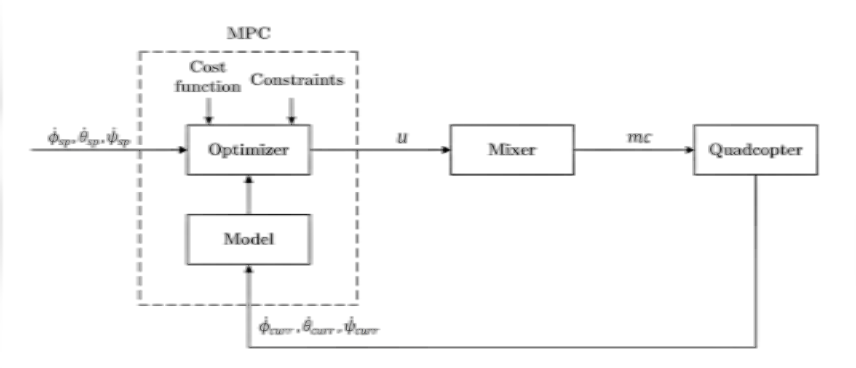
\includegraphics[width=0.8\linewidth]{./Figure/MPC-Diagram.png}
  \caption{MPC控制过程图}\label{Fig:xd1}
\end{figure}

速率设定点从姿态控制器发送到优化器块。优化器还接收成本函数和系统约束。希尔德雷斯的二次规划程序被用于优化器块,以最小化受预定义的四轴飞行器约束的成本函数。MPC控制器的输出是控制或输入向量,u。在将这个向量发布到DJI virtualstick控制之前,在-1和1之间进行缩放;这种形式的缩放是针对于DJI virtualstick控制的要求。最终将缩放后的向量发送到混控器中用于最终的四旋翼位置控制。

\chapter{实验结果}

根据实际的多次项目试飞测试,我们进行了以下的优化处理:

使用DJI飞行器传回的原始H.264视频数据进行检测处理,每帧图像耗时100ms~150ms,实时性较低,因此我们一定程度上降低了原始的H.264视频图像分辨率。

优化了无人机的控制轨迹模型,定义了更为合适的代价函数(cost function)用于将预测的输出驱动到所期望的参考值。该方法可以在样本时间k时,根据预测范围的大小生成输出预测。

\section{OpenCV视觉检测效果}

原始1080P H.264编码格式的视频逐帧处理所需时间在100ms~150ms之间,帧率约为6.7fps~10fps,难以满足实时检测的要求,而且由于该帧率下对应的控制频率在5Hz~10Hz之间,相较于期望控制频率20Hz~30Hz较低,使用PID+MPC算法进行xy位置控制存在较大的肉眼可见的比例控制振荡现象,因此我们将分辨率由1920x1080等比缩小并降低至568x320,此时的检测帧率可提升至25fps~35fps,对应的控制频率可提升至20Hz~30Hz,该控制频率下无人机的xy位置控制振荡现象明显减少,而且控制过程更为柔和。

根据二值化的阈值参数不同,以及调整霍夫圆检测中的圆心与圆心间的距离,图像中的圆的大小设置,最终将检测效果进行了一些相关优化,以下为最终的降落板识别效果:

(此处插入图片)

\section{卡尔曼滤波与优化效果}

\section{MPC模型预测控制效果}

为了验证MPC模型预测控制的效果,我们通过最小化过程通过封装Hildreth的二次规划函数和状态空间模型参数来减缓,在向混控器模块输出输入(或扭矩)命令之前至少运行两次。运行三次循环导致四轴飞行器在起飞后偏离航线,随后坠毁。然而,一个带有两次迭代的循环导致了通过每个任务路径点的相对平稳的飞行,并且任务以一个安全着陆结束。

下面绘制的飞行数据中使用的控制视野和预测视野分别为2和4。

\begin{figure}[ht]
  \centering
  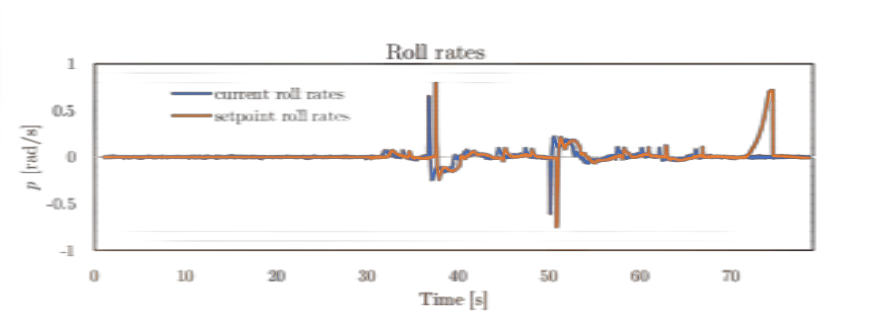
\includegraphics[width=0.8\linewidth]{./Figure/MPC-Roll-Rates.png}
  \caption{MPC滚转速率曲线}\label{Fig:xd1}
\end{figure}

\begin{figure}[ht]
  \centering
  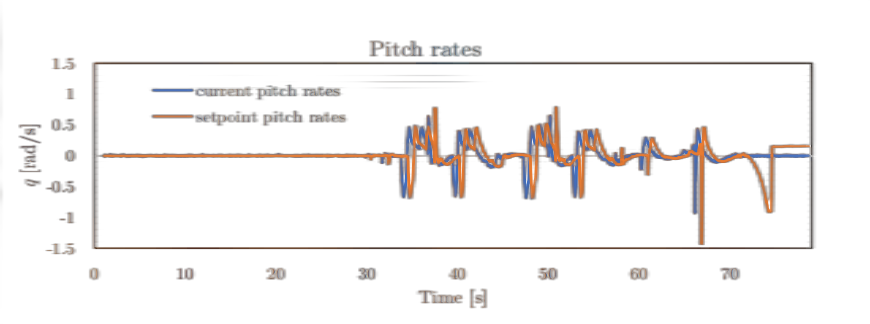
\includegraphics[width=0.8\linewidth]{./Figure/MPC-Pitch-Rates.png}
  \caption{MPC俯仰速率曲线}\label{Fig:xd1}
\end{figure}

\section{降落点精准度评价}

未使用卡尔曼滤波器的降落点检测,无人机降落落点精度为:-15cm~15cm

通过算法的优化与改进,以及添加了卡尔曼滤波器的最优估计,可以使无人机最终降落精度达到-5cm~5cm

\subsection{字体设置}
\textbf{\kaishu {西安电子科技大学}}(Xidian University)简称“\textbf{西电}”或“\textbf{西军电}”,坐落于古都西安。学校是中央部属高校,教育部直属、工信部共建,国家首批“{\heiti 211工程}”,是“{\fangsong 985工程优势学科创新平台}”、“111计划”、“2011计划”重点建设高校{\youyuan (中国电子信息领域、邮电领域唯一的“2011计划”牵头高校)},35所示范性软件学院的高校之一、集成电路人才培养基地的高校之一,56所获批设立研究生院的重点大学之一,也是{\zihao{-3}\lishu 北京高科大学联盟}的重要成员。 

1931年1月28日,红一方面军{\yahei 总司令朱德、总政委毛泽东}于小布总部签发“调学生学无线电的命令”,随后,第一期无线电训练班在\CJKunderline{小布镇陈家土楼}正式开课。后迁移至\CJKunderdblline{瑞金},成立\CJKunderwave{中央军委无线电学校},是毛泽东等老一辈革命家亲手创建的第一所工程技术学校。1958年学校迁址西安,1966年转为地方建制,1988年定为西安电子科技大学。该校是中国最早建立\CJKunderdot{信息论、信息系统工程、雷达、微波天线、电子机械、电子对抗}等专业的高校之一,开辟了中国IT学科的先河,形成了鲜明的电子与信息学科特色与优势。毛泽东曾先后两次为该校题词:“\textbf{\large 全心全意为人民服务}”、“\textbf{\large 艰苦朴素}”。\footnote{从百度百科粘下来的,就不放进参考文献了。}

\CJKsout{来点没用的}

\subsection{数字转中文}
 测试数字:1234.233. 转为中文数字:\zhnumber{1234.233};转为中文字符串:\zhdigits{1234.233}。

\section{表格}

\subsection{普通表格}
先来看一个无标题的普通表格:

\begin{tabular}{|c|c|c|}
\hline
标题 & 标题 & 标题\\
\hline
1 & 2 & 3\\
\hline
\end{tabular}

如果想要居中可以使用 \verb=center= 环境。

带标题表格。
\begin{table}[ht]
\centering
\caption{普通表格1}\label{Tab:table1}
\begin{tabular}{L{2cm}C{2cm}R{2cm}}
\hline
标题 & 标题 & 标题\\
\hline
1 & 2 & 3\\
\hline
\end{tabular}
\end{table}

来一个表格并排,每个表格一个标题:
\begin{table}[ht]
\centering
\begin{minipage}{.45\textwidth}
\centering
\caption{并排表格1}\label{Tab:table1-1}
\begin{tabular}{lcr}
\hline
标题 & 标题 & 标题\\
\hline
1 & 2 & 3\\
\hline
\end{tabular}
\end{minipage}
\begin{minipage}{.45\textwidth}
\centering
\caption{并排表格2}\label{Tab:table1-2}
\begin{tabular}{lcr}
\hline
标题 & 标题 & 标题\\
\hline
1 & 2 & 3\\
\hline
\end{tabular}
\end{minipage}
\end{table}

再来一个表格并排
\begin{table}[ht]
\centering
\caption{并排表格}
\subcaptionbox{并排表格1}
{
\begin{tabular}{lcr}
\hline
标题 & 标题 & 标题\\
\hline
1 & 2 & 3\\
\hline
\end{tabular}
}
\subcaptionbox{并排表格2}
{
\begin{tabular}{lcr}
\hline
标题 & 标题 & 标题\\
\hline
1 & 2 & 3\\
\hline
\end{tabular}
}
\end{table}


\subsection{复杂点的表格}
表 \ref{Tab:table2} 主要用到的是列合并单元格、跨行合并单元格、混合合并单元格、表格横线的自定义粗细以及控制表格横线的自定义连接等。\footnote{表格虽然难看,主要是为了让大家看效果,里面技巧选用。}
\begin{table}[ht]
\centering
\caption{复杂表格}\label{Tab:table2}
\begin{tabular}{|c|c|c|c|}
\toprule[1pt]
\multicolumn{2}{|c|}{1} & 3 & 4\\
\midrule[0.5pt]
5 & 6 & 7 & \multirow{2}*{8}\\
\cline{1-3}
9 & 10 & 11 & \\
\midrule[0.5pt]
\multicolumn{2}{|c|}{\multirow{2}*{13}} & 15 & 16\\
\cline{3-4}
\multicolumn{2}{|c|}{} & 19 & 20\\
\bottomrule[1pt]
\end{tabular}
\end{table}

表格填充颜色,如表 \ref{Tab:table3} 所示。此次,主要用到的出上述介绍外,有单个单元格填充颜色、整列填充颜色、整行填充颜色;此外,还添加了单元格划分的功能。

\begin{table}[ht]
\centering
\caption{填色表格}\label{Tab:table3}
\begin{tabular}{c | c| >{\columncolor{yellow}}c}
\toprule[1pt]
\diagbox{No.}{Title} & \textbf{L-Title} & \textbf{R-Title}\\
\hline
\rowcolor{red} 1 & One & First\\
\cellcolor[rgb]{.9,.9,.9} 2 & Two & Second\\
\cellcolor[rgb]{.2,.9,.9} 3 & Three & Third\\
\bottomrule[1pt]
\end{tabular}
\end{table}

以上,就是普通表格的常用例子了,其他的应用技巧以及功能大家自学吧,毕竟这只是个模板的使用样例,不是\LaTeX{} 教案。
\subsection{长表格}

呐,在开始长表格之前,我们应该怎么样呢?对,先说点废话。为什么呢?你想啊,既然是长表格,肯定是能够跨页存在的,不说点废话把它顶下去,顶到换页,咋能对得起它的NB功能呢,是吧。

咳咳,严肃点,主角登场了。表 \ref{Tab:longtable} 就是这一小节的主角——长表格了。首先说明一下,这种表格如果放的数据太多的话,就不要在正文里面用了,放到附录里就可以了。

\begin{longtable}[c]{cC{2cm}C{2cm}C{2cm}C{2cm}}
\caption{这是一个长表格}\label{Tab:longtable}\\
\hline
行号 & 标题1 & 标题2 & 标题3 & 标题4\\
\hline
\endfirsthead %以上是最前的表头
\multicolumn{5}{c}{\zihao{5}续表 \thetable\quad 这是一个长表格}\\
\hline
行号 & 标题1 & 标题2 & 标题3 & 标题4\\
\hline
\endhead %以上是换页后的表头,如未换页,并不会显示
\hline
\multicolumn{5}{r}{接下页续表……}\\
\endfoot %以上是前页的表尾,如未换页,并不会显示。
\hline
\endlastfoot%以上选填最后也的表尾。一般不填
%下面开始长表格的内容
1 & 1 & 2 & 3 & 4\\
2 & 5 & 6 & 7 & 8\\
3 & 9 & 10 & 11 & 12\\
4 & 13 & 14 & 15 & 16\\
5 & 17 & 18 & 19 & 20\\
6 & 21 & 22 & 23 & 24\\
7 & 25 & 26 & 27 & 28\\
8 & 29 & 30 & 31 & 32\\
9 & 33 & 34 & 35 & 36\\
10 & 37 & 38 & 39 & 40\\
11 & 41 & 42 & 43 & 44\\
12 & 45 & 46 & 47 & 48\\
13 & 49 & 50 & 51 & 52\\
14 & 52 & 54 & 55 & 56\\
15 & 57 & 58 & 59 & 60\\
16 & 61 & 62 & 63 & 64\\
17 & 65 & 66 & 67 & 68\\
18 & 69 & 70 & 71 & 72\\
19 & 73 & 74 & 75 & 76\\
20 & 77 & 78 & 79 & 80\\
21 & 81 & 82 & 83 & 84\\
22 & 85 & 86 & 87 & 88\\
23 & 89 & 90 & 91 & 92\\
24 & 93 & 94 & 95 & 96\\
25 & 97 & 98 & 99 & 100\\
\end{longtable}

\section{图片}
\subsection{普通图片的插入}
如同表格一样,插图一般都用浮动体来控制,这样排出来的文章美观。\footnote{本文涉及到的所有图片,除我校校徽等标记外,均为个人拍摄。}比如,图 \ref{Fig:xd1} 所示,是一个图片的样例。
\begin{figure}[ht]
  \centering
  \includegraphics[width=0.8\linewidth]{./Figure/IMG_XD1.jpg}
  \caption{西电1}\label{Fig:xd1}
\end{figure}

\subsection{图片并排插入}

先来看第一个,两个图片分别一个标题,如图 \ref{Fig:xd2} 和 图 \ref{Fig:xd3}.
\begin{figure}[ht]
\centering
\begin{minipage}{.45\textwidth}
\centering
\includegraphics[width=1\linewidth]{./Figure/IMG_XD2.jpg}
  \caption{西电2}\label{Fig:xd2}
\end{minipage}~
\begin{minipage}{.45\textwidth}
\centering
\includegraphics[width=1\linewidth]{./Figure/IMG_XD3.jpg}
  \caption{西电3}\label{Fig:xd3}
\end{minipage}
\end{figure}

再来看一个统一大标题带子标题的,如图 \ref{Fig:bingpai} 所示。
\begin{figure}[ht]
\centering
\subcaptionbox{西电4}
{\includegraphics[width=.45\linewidth]{./Figure/IMG_XD4.jpg}}
\subcaptionbox{西电5}
{\includegraphics[width=.45\linewidth]{./Figure/IMG_XD5.jpg}}
\caption{并排插图}\label{Fig:bingpai}
\end{figure}

插图就介绍到这,其他知识自学。

\section{公式}
\subsection{普通公式}
先来看一个行内公式:$y=x+1$.

下面是一个居中的公式:
\[
f(X)=\sum_{i=1}^{n}\sin{\frac{\pi}{2}x_i}
\]

看一个编号的公式,如式\eqref{Eq:eq1}:
\begin{equation}\label{Eq:eq1}
f(X)=\sum_{i=1}^{n}\sin{\frac{\pi}{2}x_i}
\end{equation}

\subsection{复杂公式}
\begin{itemize}
\item \textbf{多行公式}

\begin{equation}\label{Eq:eq2}
\begin{aligned}
f(x) &= \sin(a+b)\\
&= \sin(a)\cos(b)+\cos(a)\sin(b).
\end{aligned}
\end{equation}

\begin{equation}\label{Eq:eq3}
f(x) = \left\{
\begin{aligned}
 -&x+1,\quad \text{if}~x<0;\\
 &x+1,\quad \text{if}~x \geq 0;
 \end{aligned}
 \right.
\end{equation}

\item \textbf{矩阵}

\[
  A = \left(\begin{array}{ccc}
        a_{11} & a_{12} & a_{13} \\
        a_{21} & a_{22} & a_{23} \\
        a_{31} & a_{32} & a_{33}
      \end{array}\right),\quad
  B = \left[\begin{array}{ccc}
        b_{11} & b_{12} & b_{13} \\
        b_{21} & b_{22} & b_{23} \\
        b_{31} & b_{32} & b_{33}
      \end{array}\right],\quad
   C = \left[\begin{array}{ccc}
     c_{11} & c_{12} & c_{13} \\
     \vdots & \ddots & \vdots \\
     c_{31} & c_{32} & c_{33}
   \end{array}\right].
\]
行列式也类似
\[
A = \left|\begin{array}{ccc}
    a_{11} & a_{12} & a_{13} \\
    a_{21} & a_{22} & a_{23} \\
    a_{31} & a_{32} & a_{33}
  \end{array}\right|.
\]

\item \textbf{其他公式}

\[
\mathbb{L} = \int_{x_1}^{x_2}\sqrt{1+(y')^2}dx 
= \frac{1}{\alpha}\int_{x_1}^{x_2}y''(x)dx
\]

\end{itemize}

\section{休息一下}

\subsection{山水之间}
\begin{center}
\textbf{山水之间}

{\kaishu 许嵩}

\vspace*{1em}
昨夜同门云集\quad 推杯又换盏\\
今朝茶凉酒寒\quad 豪言成笑谈\\
半生累\quad 尽徒然\\
碑文完美有谁看\\
隐居山水之间\quad 誓与浮名散\\

\vspace*{.6em}
湖畔青石板上\quad 一把油纸伞\\
旅人停步折花\quad 淋湿了绸缎\\
满树玉瓣多傲然\\
江南烟雨却痴缠\\
花飞雨追\quad 一如尘缘理还乱\\

\vspace*{.6em}
落花雨\quad 你飘摇的美丽\\
花香氤\quad 把往日情勾起\\
我愿意\quad 化浮萍躺湖心\\
只陪你\quad 泛岁月的涟漪
\end{center}

\subsection{念奴娇·赤壁怀古}

\begin{center}
\textbf{念奴娇·赤壁怀古}

{\kaishu 苏轼}

\vspace*{1em}
大江东去,浪淘尽,千古风流人物。\\
故垒西边,人道是:三国周郎赤壁。\\
乱石穿空,惊涛拍岸,卷起千堆雪。\\
江山如画,一时多少豪杰。\\

\vspace*{.8em}
遥想公瑾当年,小乔初嫁了,雄姿英发。\\
羽扇纶巾,谈笑间樯橹灰飞烟灭。\\
故国神游,多情应笑我,早生华发。\\
人生如梦,一尊还酹江月。

\end{center}

这一章就写到这里吧,下一章重点介绍两个内容

\chapter{两个重点}
这一章,会涉及到环境以及参考文献两个重点东西。

\section{环境}
\subsection{定理类环境}

\begin{proposition}\label{prop:p1}
这是一个命题。
\end{proposition}

它还可以这么写,所有定理类环境,都可这么写。

\begin{proposition}[命题名]
由命题 \ref{prop:p1}, 这也是一个命题。
\end{proposition}

\begin{assumption}
距离水平面$100\,m$以内,重力加速度$g$是不变的。
\end{assumption}

\begin{lemma}[法图引理]
设$(S,\Sigma,\mu)$为一个测度空间,$(f_n)_{n\geq 0}$是一个实值的可\textbf{正值}函数列。那么:
\[
\int_S \liminf_{n\rightarrow \infty} f_n d\mu \leqslant \liminf_{n\rightarrow \infty} \int_S f_n d\mu.
\]
其中函数极限是在逐点收敛的意义上的极限,函数取值和积分可以是无限大的。
\end{lemma}

\begin{theorem}
若$\lim_{n\rightarrow \infty} x_n = a$,则$\{x_n\}$的任何子列$\{x_{n_k}\}$都收敛于$a$.
\end{theorem}
\begin{proof}
因$\lim_{n\rightarrow \infty} x_n = a$,对任意给定的$\varepsilon > 0$,必定存在正整数$N$,当$n>N$时,有
\[
|x_n-a|<\varepsilon.
\]
今取$K=N$,则对一切$k>K$,有$n_k>n_K=n_N\geq N$,这时就有
\[
|x_{n_k} - a|<\varepsilon.
\]
\end{proof}

\subsection{算法环境}
如算法 \ref{euclid} 所示,详细使用方法见文档 \href{https://ctan.org/pkg/algorithmicx?lang=en}{algorithmicx} (此条参考自\href{https://github.com/mohuangrui/ucasthesis}{中国科学院大学学位论文 LaTeX 模板})
\begin{algorithm}
    \caption{Euclid’s algorithm}\label{euclid}
    \begin{algorithmic}[1]
    \Procedure{Euclid}{$a,b$}\Comment{The g.c.d. of a and b}
    \State $r\gets a\bmod b$
    \While{$r\not=0$}\Comment{We have the answer if r is 0}
    \State $a\gets b$
    \State $b\gets r$
    \State $r\gets a\bmod b$
    \EndWhile\label{euclidendwhile}
    \State \textbf{return} $b$\Comment{The gcd is b}
    \EndProcedure
    \end{algorithmic}
\end{algorithm}

\subsection{代码环境}

\begin{lstlisting}[language=C]
#include<stdio.h>

int main()
{
	printf("Hello World!");
	return 0;
}
\end{lstlisting}

\begin{lstlisting}[language=C,caption={Java代码},label=Code:java]
package com.stick.test;

/**
 * 公共主类;
 * 类名必须与文件名相同
 */
public class Test{
	public static void main(String[] args) {
		System.out.println("Hello World!");
	}
}
\end{lstlisting}

\begin{lstlisting}[language=R,style = nonumbers]
x<-c(1,2,3,4,5,6)
y<-sin(x)
lines(x,y)
\end{lstlisting}
\section{参考文献的引用}
以下为常用的参考文献。

期刊\cite{Art,ArtE},专著(无页码)\cite{Boo,BooE,Boo1},专著(含页码)\cite{InBoo,InBoo1,InBooE},论文集\cite{Incol,IncolE}。

硕士\cite{MT}/博士论文\cite{Phd},科技报告\cite{TechR}。

以下参考文献,原有plain风格中并无,为Stick本人自己写的。

网络内容引用\cite{Net},译著\cite{Trans}

此外,多说一句,本文模板加载的 \verb=natbib= 宏包使得 \verb=\cite= 命令还支持排序等功能。

比如下列文献\cite{ArtE,BooE,InBooE,Trans,Net}